\chapter{\bf{State Diagram}}
\boldmath

\section{Input, Output e Stati}

Lo \textbf{state diagram} è una rappresentazione grafica che mostra i differenti stati in cui un sistema può trovarsi e le transizioni tra questi ultimi, in funzione di variabili esterne.

\vspace{3mm}

\noindent Gli input del diagramma principale sono:

\begin{itemize}
    \item \textbf{B1}: bottone per la chiusura e apertura del cancello
    \item \textbf{B2}: bottone per la regolazione del tempo di chiusura automatica del cancello
    \item \textbf{B3}: bottone per la regolazione del tempo di lavoro del cancello
    \item \textbf{P1}: sensore di presenza per la rilevazione di ostacoli
    \item \textbf{P2}: sensore di presenza per la rilevazione della chiusura completa del cancello
    \item $T_L$: timer relativo al tempo di lavoro
    \item $T_C$: timer relativo al tempo di chiusura automatica
\end{itemize}

\noindent Gli output del diagramma sono:

\begin{itemize}
    \item \textbf{Led Green}
    \item \textbf{Led Yellow}
    \item \textbf{Led Red}
\end{itemize}

\noindent Gli stati del diagramma sono:

\begin{itemize}
    \item \textbf{Inattivo:} è lo stato iniziale del sistema, disponibile appena dopo l'accensione, durante il quale viene controllata l'attivazione dei due sensori di presenza $P1$ e $P2$ per garantire una corretta chiusura del cancello dopo l'accensione dello stesso;

    \item \textbf{Chiusura:} macrostato esterno che raggruppa al suo interno:
        \begin{itemize}
            \item \textbf{In Chiusura:} raffigura lo stato secondo cui il cancello si sta chiudendo, durante il quale si controlla l'eventuale presenza di ostacoli. Si controlla anche che il cancello si chiuda entro il tempo di lavoro ($T_L$) prestabilito;
        
            \item \textbf{Chiuso:} rappresenta lo stato per cui il cancello risulta completamente chiuso;

            \item \textbf{Errore:} macrostato relativo alla gestione degli errori, suddiviso in:

            \begin{itemize}
                \item \textbf{In Errore:} simboleggia lo stato di errore che si verifica nel momento in cui il cancello risulta non chiuso dopo il tempo prestabilito ($T_L$);

                \item \textbf{LED Rosso Errore:} simboleggia lo stato in cui il dispositivo entra quando il cancello risulta non chiuso dopo il tempo prestabilito ($T_L$) più 10 secondi di attesa. È connotato dall'accensione del LED rosso.
            \end{itemize}
        \end{itemize}
    
    \item \textbf{Apertura:} macrostato contenente i seguenti stati:
        \begin{itemize}
            \item \textbf{In Apertura:} delinea lo stato di apertura in corso del cancello;
    
            \item \textbf{Aperto:} rappresenta lo stato in cui il cancello risulta completamente aperto;
        \end{itemize}

    \item \textbf{Ostacolo:} macrostato relativo alla gestione degli ostacoli. Gli stati interni sono:
        \begin{itemize}
            \item \textbf{Fermo:} rappresenta lo stato di attesa in cui si trova il cancello prima dell'attivazione del pulsante $B1$ e/o dopo lo scadere dei 30 secondi di \textit{blinking} del LED verde o dopo la rimozione dell'ostacolo;
        
            \item \textbf{Ostacolo presente:} descrive lo stato durante il quale il cancello è aperto/chiuso/inattivo ma è stata rilevata la presenza di un ostacolo dal sensore $P1$ e, dunque, non vi è possibilità di movimento;
        \end{itemize}

    \item \textbf{Regolazioni:} macrostato contenente gli stati addetti alla regolazione dei tempi di chiusura ($T_C$) e di lavoro ($T_L$). Contiene:
        \begin{itemize}
            \item \textbf{Tempo Lavoro:} imposta il tempo di lavoro iniziale ad una quantità pari a 10 secondi;

            \item \textbf{Aggiunta Tempo Lavoro:} incrementa il tempo di lavoro di 10 secondi ad ogni interazione fino al raggiungimento dei 120 secondi, dopo i quali riparte da 10;

            \item \textbf{Tempo Chiusura:} imposta il tempo di chiusura iniziale ad una quantità pari a 10 secondi;

            \item \textbf{Aggiunta Tempo Chiusura:} incrementa il tempo di chiusura di 10 secondi ad ogni interazione fino al raggiungimento dei 120 secondi, dopo i quali riparte da 10.
        \end{itemize}
\end{itemize}

\vspace{10mm}

\begin{figure}[H]
    \centering
    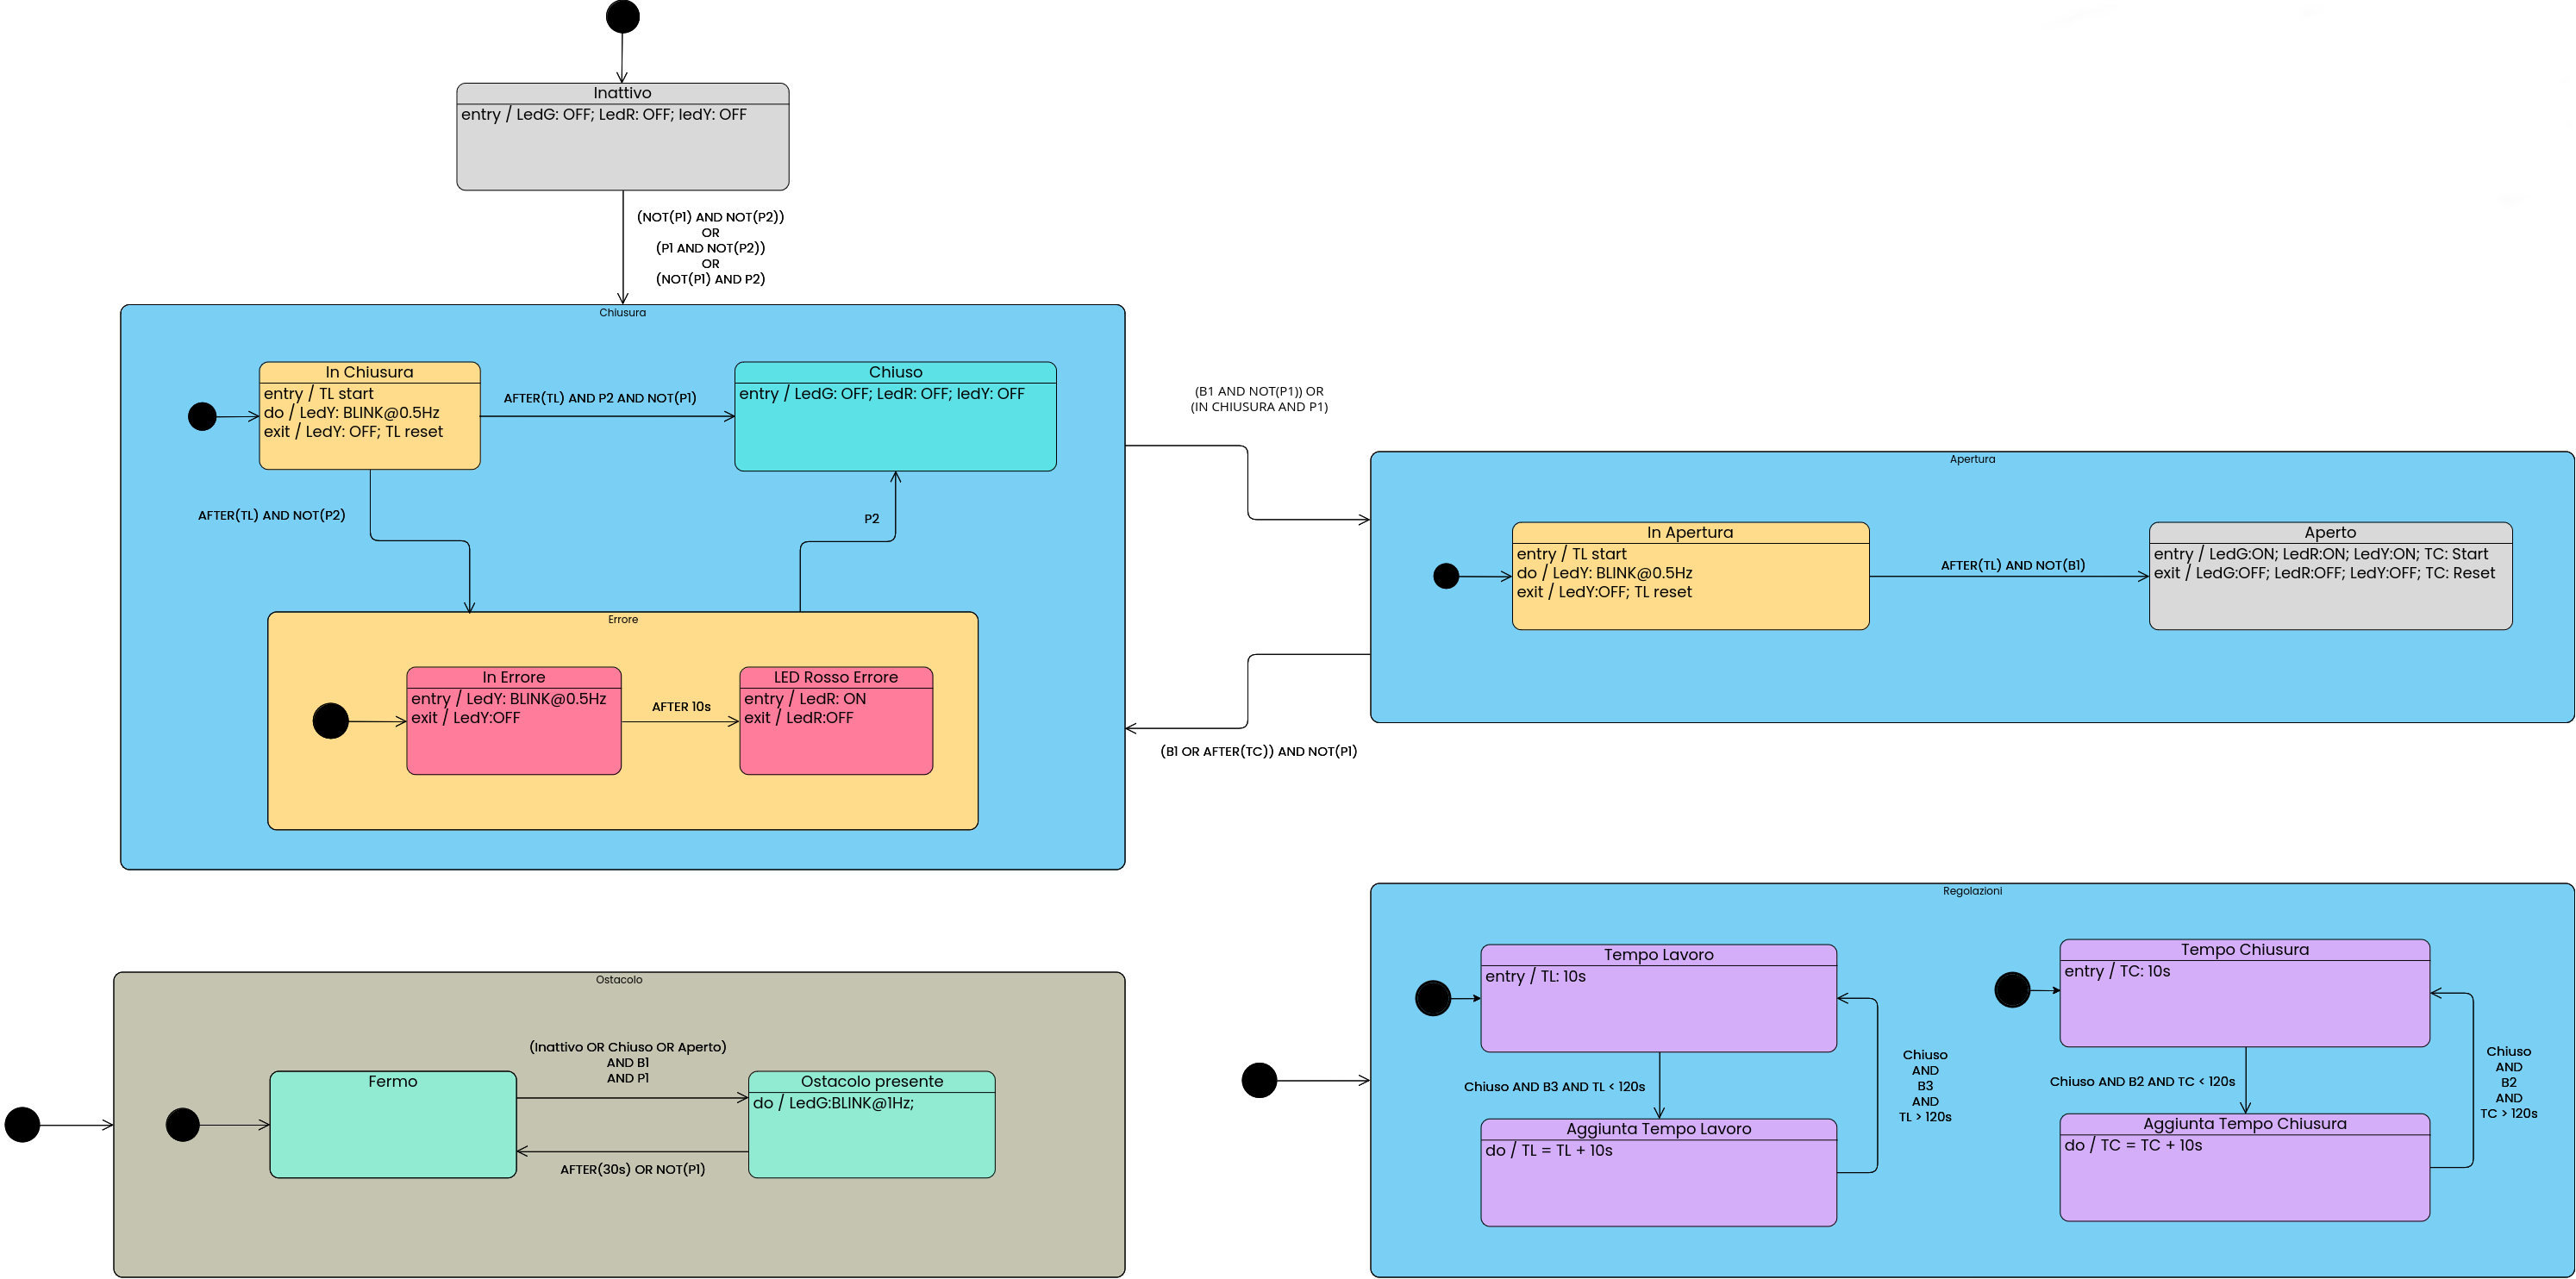
\includegraphics[width=0.9\textwidth]{figures/statediagram.png}
    \caption{State Diagram}
    \label{state}
\end{figure}


\section{Logica di Funzionamento}

\subsection{Stato \textit{Inattivo}}
    All'avvio, il sistema si trova nello stato iniziale \textbf{Inattivo}, durante il quale si controlla lo stato dei due sensori di presenza $P1$ e $P2$, al fine di ritornare allo stato iniziale desiderato di \textbf{Chiuso}.
    
    \noindent Le transizioni in uscita da esso prevedono, per progettazione, il passaggio nel macrostato \textit{Chiusura} e sono:
    
    \begin{itemize}
        \item se entrambi i sensori sono disattivati si procede alla chiusura passando allo stato \textbf{In Chiusura};
        
        \item se è attivo il sensore di presenza $P1$, ma non il sensore $P2$, si passa per lo stato \textbf{In Chiusura} per poi giungere subito allo stato \textbf{In Apertura}, contenuto nel macrostato \textit{Apertura};
        
        \item se non è attivo il sensore di presenza $P1$, ma lo è $P2$, si giunge allo stato \textbf{Chiuso} per segnalarne la corretta chiusura;
    \end{itemize}


\subsection{Macrostato \textit{Chiusura}}
    All'interno del macrostato in esame sono presenti diverse strutture, in particolare due stati interni (\textbf{In Chiusura} e \textbf{Chiuso}) e un macrostato sottostante \textbf{Errore} (quest'ultimo analizzato nel \hyperref[macrostato-errore]{paragrafo 4.2.3}).
    
    \noindent La transizione in uscita da questo macrostato è la seguente:
    \begin{itemize}
        \item \textit{Chiusura $\rightarrow$ Apertura:} se l'utente preme il bottone $B1$ senza che vi sia la rilevazione di ostacoli dal sensore $P1$ o se viene rilevato un ostacolo senza la pressione del pulsante mentre si è nello stato \textbf{In Chiusura}, si passa al macrostato \textbf{Apertura};
    \end{itemize}

    \noindent Di seguito sono trattati gli stati interni.

    \subsubsection{Stato \textit{In Chiusura}}
    In questo stato viene innanzitutto iniziato il conteggio del timer relativo al tempo di lavoro ($T_L$).
    Durante la persistenza dello stato, viene inoltre attivato il \textit{blink} del LED giallo ad una frequenza pari a 0.5Hz per segnalare il movimento del cancello. All'uscita dallo stato, il LED giallo viene spento e il timer di $T_L$ viene resettato.
    
    \noindent Le transizioni in uscita da questo stato sono:
    \begin{itemize}
        \item \textit{In Chiusura $\rightarrow$ Chiuso:} se termina il tempo di lavoro ($T_L$) e si attiva il sensore di presenza $P2$ e non vi è rilevazione di ostacoli dal sensore $P1$, allora si passa allo stato \textbf{Chiuso};
        
        \item \textit{In Chiusura $\rightarrow$ Errore:} se dovesse scadere il tempo di lavoro ($T_L$), ma senza alcuna attivazione del sensore di presenza $P2$, si passerebbe al macrostato di \textbf{Errore}.
    \end{itemize}

    \subsubsection{Stato \textit{Chiuso}}
    Questo stato interno rappresenta lo stato di chiusura avvenuta del cancello, rilevata dall'attivazione del sensore $P2$.
    Non vi sono transizioni in uscita e l'unica azione effettuata da questo stato è quella di spegnere tutti i LED.


\subsection{Macrostato \textit{Errore}} \label{macrostato-errore}
    Nel macrostato attuale, contenuto nel macrostato esterno \textbf{Chiusura}, ci si occupa della gestione dello stato di errore, nello specifico sono presenti due stati interni (\textbf{In Errore} e \textbf{LED Rosso Errore}) 

    \noindent L'unica transizione in uscita è:
    \begin{itemize}
        \item \textit{Errore $\rightarrow$ Chiuso:} se il sensore $P2$ rileva l'avvenuta chiusura del cancello è possibile uscire dallo stato di errore.
    \end{itemize}
    
    \noindent Di seguito sono trattati gli stati interni.
        
    \subsubsection{Stato \textit{In Errore}}
        In questo stato è ancora presente il \textit{blinking} del LED giallo ad una frequenza di 0.5Hz, il quale viene spento soltanto all'uscita. È possibile entrare nel poc'anzi citato stato nel momento in cui scade la durata del tempo di lavoro ($T_L$) e non vi è ancora alcuna segnalazione da parte del sensore di chiusura $P2$.
        
        \noindent La transizione in uscita è:
        \begin{itemize}
            \item \textit{In Errore $\rightarrow$ LED Rosso Errore:} se dopo la scadenza del tempo di lavoro ($T_L$) e una successiva attesa di 10 secondi, non è stata ancora segnalata la chiusura dal sensore $P2$, allora si entra nello stato \textbf{LED Rosso Errore}.
        \end{itemize}

    \subsubsection{Stato \textit{LED Rosso Errore}}
        Quando si entra in questo stato avviene l'accensione del LED rosso, a indicare che sono trascorsi 10 secondi dalla scadenza del tempo di lavoro ($T_L$) e non è ancora pervenuta nessuna segnalazione da parte del sensore di chiusura ($P2$).
        Non sono presenti transizioni in uscita da questo stato.

\subsection{Macrostato \textit{Apertura}}
    Nel macrostato di cui si sta trattando ora, è possibile osservare l'esistenza di due stati interni (\textbf{In Apertura} e \textbf{Aperto}).
    
    \noindent L'unica transizione in uscita è:
    \begin{itemize}
        \item \textit{Apertura $\rightarrow$ Chiusura:} se l'utente preme il bottone $B1$ o se scade il tempo di chiusura ($T_C$) senza che vi sia la rilevazione di un ostacolo da parte del sensore $P1$, allora si entra nel macrostato \textbf{Chiusura}.
    \end{itemize}

    \noindent Di seguito sono trattati gli stati interni.
    
    \subsubsection{Stato \textit{In Apertura}}
        In questo stato viene dapprima avviato il conteggio del timer relativo al tempo di lavoro ($T_L$).
        Durante la persistenza dello stato, viene inoltre attivato il \textit{blink} del LED giallo ad una frequenza pari a 0.5Hz per segnalare il movimento del cancello. All'uscita dallo stato, viene spento il LED giallo e si resetta il timer $T_L$.
        
        \noindent La transizione in uscita da questo stato è la seguente:
        \begin{itemize}
            \item \textit{In Apertura $\rightarrow$ Aperto:} se dovesse scadere il tempo di lavoro ($T_L$) senza alcuna pressione del bottone $B1$, si entrerebbe nello stato \textbf{Aperto}.
        \end{itemize}

    \subsubsection{Stato \textit{Aperto}}
        Nello stato in essere vengono accesi staticamente tutti i LED per segnalare la corretta apertura del cancello ed inoltre viene attivato anche il timer relativo alla chiusura ($T_C$). Inoltre, non sono presenti transizioni in uscita dallo stato, ma in uscita dallo stesso vengono spenti tutti i LED e il timer del tempo di chiusura ($T_C$) viene resettato.


\subsection{Macrostato \textit{Ostacolo}}
    In questo macrostato ci sono due stati interni (\textbf{Fermo} e \textbf{Ostacolo}), oltretutto non sono presenti transizioni in uscita.

    \noindent Di seguito sono trattati gli stati interni.
    
    \subsubsection{Stato \textit{Fermo}}
        Questo stato indica che il sistema attende la pressione del pulsante $B1$ da parte dell'utente.
        Ci si trova in questo stato quando o il cancello è inattivo/chiuso/aperto o dopo che sono trascorsi 30 secondi di lampeggio del LED verde o dopo la rimozione dell'ostacolo dalla fotocellula $P1$.
        
        \noindent La transizione in uscita è:
        \begin{itemize}
            \item \textit{Fermo $\rightarrow$ Ostacolo presente:} se il dispositivo si trova nello stato \textit{Inattivo} o \textit{Chiuso} o \textit{Aperto} e l'utente preme il bottone $B1$ in presenza di ostacolo, rilevato dal sensore $P1$, si passa allo stato \textbf{Ostacolo presente}.
        \end{itemize} 

    \subsubsection{Stato \textit{Ostacolo presente}}
        Questo stato si occupa della gestione del LED verde, attivandone il \textit{blinking} ad una frequenza di 1Hz fintantoché l'ostacolo è presente dinanzi alla fotocellula $P1$ per un massimo di 30 secondi.

        \noindent La transizione in uscita è:
        \begin{itemize}
            \item \textit{Ostacolo presente $\rightarrow$ Fermo:} si passa allo stato \textbf{Fermo} una volta passati i 30 secondi di \textit{blinking} del LED verde o nel momento in cui l'ostacolo non viene più rilevato.
        \end{itemize}


\subsection{Macrostato \textit{Regolazioni}}
    In questo macrostato l'utente può regolare sia il tempo di chiusura ($T_C$) che il tempo di lavoro ($T_L$) tramite, rispettivamente, la pressione dei bottoni $B2$ e $B3$, modificandone la durata in un range che spazia dai 10 secondi ai 120 secondi. Non vi sono transizioni in uscita e la pressione dei due bottoni $B2$ e $B3$ è ignorata in tutti gli altri stati.

    \noindent Di seguito sono analizzati gli stati interni.

    \subsubsection{Tempo di Chiusura}
        \begin{itemize}
            \item \textbf{Stato \textit{Tempo Chiusura}} \\
                L'azione principale di questo stato è impostare il tempo di chiusura ($T_C$) a 10 secondi.
                \noindent La transizione in uscita è:
                \begin{itemize}
                    \item \textit{Tempo Chiusura $\rightarrow$ Aggiunta Tempo Chiusura:} se il cancello si trova nello stato \textbf{Chiuso}, l'utente preme il bottone $B2$ e il tempo di chiusura ($T_C$) attuale è inferiore a 120 secondi, allora si entra nello stato \textbf{Aggiunta Tempo Chiusura}.
                \end{itemize}

            \item \textbf{Stato \textit{Aggiunta Tempo Chiusura}} \\
                In questo stato si incrementa, ad ogni iterazione, la durata del tempo di chiusura ($T_C$) di 10 secondi.
                \noindent La transizione in uscita è:
                \begin{itemize}
                    \item \textit{Aggiunta Tempo Chiusura $\rightarrow$ Tempo Chiusura:} se il cancello è \textbf{Chiuso}, l'utente preme il bottone $B2$ e il tempo di chiusura ($T_C$) attuale è uguale a 120 secondi, anziché aumentare, esso viene ripristinato a 10 secondi entrando nello stato \textbf{Tempo Chiusura}.
                \end{itemize}
        \end{itemize}

    \subsubsection{Tempo di Lavoro}
        \begin{itemize}
            \item \textbf{Stato \textit{Tempo Lavoro}} \\
                L'azione principale di questo stato è impostare il tempo di lavoro ($T_L$) a 10 secondi.
                \noindent La transizione in uscita è:
                \begin{itemize}
                    \item \textit{Tempo Lavoro $\rightarrow$ Aggiunta Tempo Lavoro:} se il cancello si trova nello stato \textbf{Chiuso}, l'utente preme il bottone $B3$ e il tempo di lavoro ($T_L$) attuale è inferiore a 120 secondi, allora si entra nello stato \textbf{Aggiunta Tempo Chiusura}.
                \end{itemize}

            \item \textbf{Stato \textit{Aggiunta Tempo Lavoro}} \\
                In questo stato si incrementa, ad ogni iterazione, la durata del tempo di lavoro ($T_L$) di 10 secondi.
                \noindent La transizione in uscita è:
                \begin{itemize}
                    \item \textit{Aggiunta Tempo Lavoro $\rightarrow$ Tempo Lavoro:} se il cancello si trova nello stato \textbf{Chiuso}, l'utente preme il bottone $B3$ e il tempo di lavoro ($T_L$) attuale è uguale a 120 secondi, allora si entra nello stato \textbf{Tempo Lavoro}.
                \end{itemize}
        \end{itemize}